
% Prepared by Calvin Kent
%
% Assignment Template v19.02
%
%%% 20xx0x/MATHxxx/Crowdmark/Ax
%
\documentclass[12pt]{article} %
\usepackage{CKpreamble}
\usepackage{CKassignment}
\usepackage{tkz-euclide}
\usepackage{physunits}
\usepackage{physics}
\usepackage{lmodern}
\usepackage{microtype}
\usepackage{upgreek}
\usepackage[misc]{ifsym}
\title{\textbf{Functions 11 Unit 1 Diagnostic} \\ \emph{Due: Monday, November 28} \\ \emph{Not being Graded}}
\date{2021\\ November}
\author{Abdullah Zubair}

%%% Maths and science packages

\usepackage{amsmath,amsthm,amssymb}
\pgfplotsset{my style/.append style={axis x line=middle, axis y line=
middle, xlabel={$x$}, ylabel={$y$}, axis equal }}
\usepackage{pgfplots}
	\usetikzlibrary{
		calc,
		patterns,
		positioning
	}
	\pgfplotsset{
		compat=1.16,
		samples=200,
		clip=false,
		my axis style/.style={
			axis x line=middle,
			axis y line=middle,
			legend pos=outer north east,
			axis line style={
				->,
			},
			legend style={
				font=\footnotesize
			},
			label style={
				font=\footnotesize
			},
			tick label style={
				font=\footnotesize
			},
			xlabel style={
				at={
					(ticklabel* cs:1)
				},
				anchor=west,
				font=\footnotesize,
			},
			ylabel style={
				at={
					(ticklabel* cs:1)
				},
				anchor=west,
				font=\footnotesize,
			},
			xlabel= $x$,
			ylabel=$\vec d (\m \tx{[East]})$
		},
	}
	\tikzset{
		>=stealth
	}

%%% Tables and figures packages

\usepackage{float}
\usepackage{caption}
	\captionsetup{
		format=plain,
		labelfont=bf,
		font=small,
		justification=centering
	}
	
%%% Numbers and sets

\newcommand{\E}{\mathrm{e}}

\newcommand{\tx}[1]{\text{#1}}

\begin{document}
    \pagenumbering{arabic}
    % Start of class settings ...
    \renewcommand*{\coursecode}{Diagnostic} % renew course code
    \renewcommand*{\assgnnumber}{Unit 1} % renew assignment number
    \renewcommand*{\submdate}{November 22, 2021} % renew the date
    \renewcommand*{\studentfname}{Functions} % Student first name
    \renewcommand*{\studentlname}{11} % Student last name
    %\renewcommand*{\studentnum}{SNumber} % Student number

    \renewcommand\qedsymbol{$\blacksquare$}
    \setfigpath
    % End of class settings 
    \pagestyle{crowdmark}
    \newgeometry{left=18mm, right=18mm, top=22mm, bottom=22mm} % page is set to default values
    \fancyhfoffset[L,O]{0pt} % header orientation fixed
    % End of class settings
    %%% Note to user:
    % CTRL + F <CHANGE ME:> (without the angular brackets) in CKpreamble to specify graphics paths accordingly.
    % The command \circled[]{} accepts one optional and one mandatory argument.
    % Optional argument is for the size of the circle and mandatory argument is for its contents.
    % \circled{A} produces circled A, with size drawn for letter A. \circled[TT]{A} produces circled A with size drawn for TT.
    % https://github.com/CalvinKent/My-LaTeX
    %%%
    % Crowdmark assignment start


    %%%%%%%%%%%%%%%%%% PROBLEMS IDEAS %%%%%%%%%%%%%%%%%%%%%%%%%%%%%%%%%%%%%%%%%
	%% --> Half circle problem
    %% --> System of equations
    %% --> Comparing two motions, time difference
    %% --> Relative vector problem with at least 4 points
	%% --> REDO Q8 from review and this time ask him to compute the speed required.
	%% --> Problem related to question 8 from HW3 to test him


	\maketitle \section{Preamble} This is a a diagnostic assignment for our first unit in the course. It will test you on material that
	you should know prior to Unit 1. \emph{Show all of your work} when presenting their final solutions.\\
	\textbf{Note:} Some problems will refer you to the textbook.
	 \section{Name and Date:} Print your name and todays date below;\\


	\begin{center} \noindent\begin{tabular}{ll} \makebox[3in]{\hrulefill} & \makebox[3in]{\hrulefill}\\ Name & Date\\[8ex]% adds space
	 \end{tabular} \end{center} \newpage

%%%%%%%%%%%%%%%%%%%%%%%%%%%%%%%%%%%%%%%%%%%%%%%%%%%%%%%%%%%%%%%%%%%%%%%%%%%%%%%%%%%%%%%%%%%
	 %%% Problems 
%%%%%%%%%%%%%%%%%%%%%%%%%%%%%%%%%%%%%%%%%%%%%%%%%%%%%%%%%%%%%%%%%%%%%%%%%%%%%%%%%%%%%%%%%%%
	 

\begin{qstn}[1] Sketch each linear relation on the plot below, make sure to label each graph, as well as \emph{at least one point} . The graph
	does \emph{not} have to be to scale. I have provided an example as reference.
	\begin{enumerate}[label = (\alph*)]
		\item $y = 3x - 1$
		\item $y = \frac{-1}{4}x + 5$
		\item $y = 6$
		\item $2x - 3y + 12 = 0$
	\end{enumerate}
	 \begin{center}
			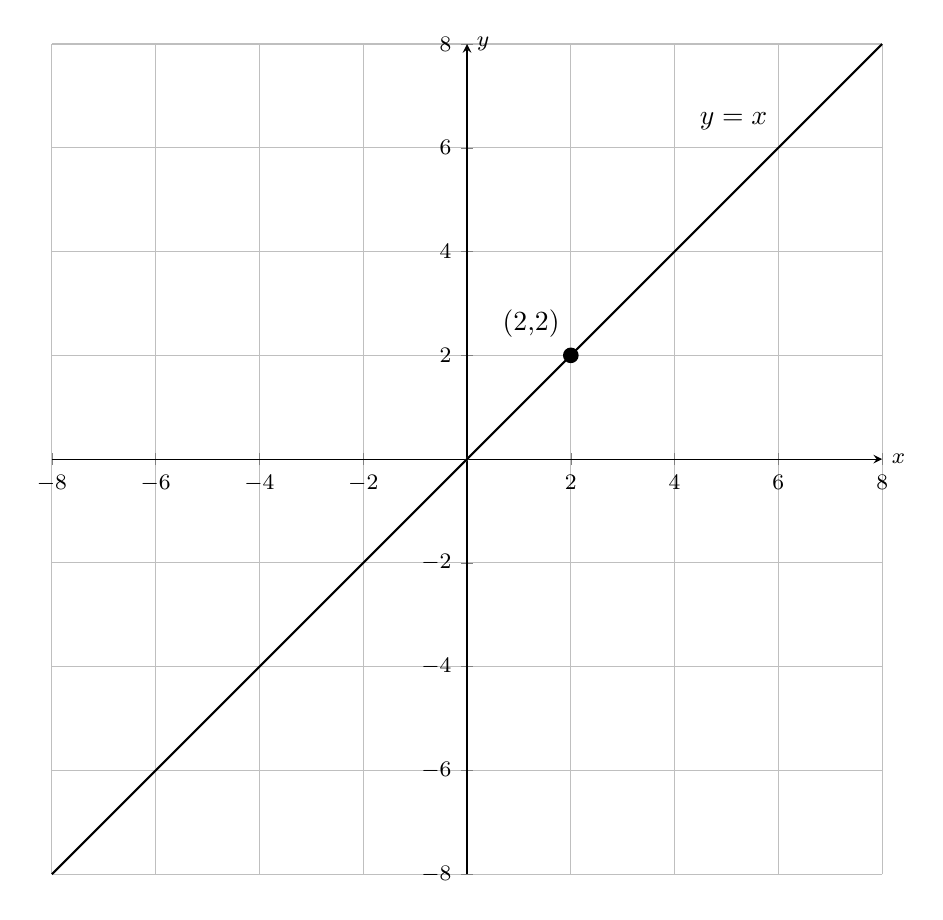
\begin{tikzpicture} \begin{axis}[ my axis style, width=\textwidth, height=\textwidth, ylabel=$y$, grid ]
	
			\addplot[ domain=-8:8, thick, white, - ] {x};
			\addplot[ domain=-8:8, thick, black, - ] {x};

				\node[label={100:{($2$,2)}},circle,fill,inner sep=2pt] at (axis cs:2,2) {};
				\node[label={100:{$y = x$}},circle,inner sep=2pt] at (axis cs:6,6) {};
        
			
			\fill[ black ];
			
			\end{axis} \end{tikzpicture}
 \end{center}
 \newpage
 \textbf{Problem 2: Textbook, Pg 2: } Question 2.\\
 \\
 \textbf{Problem 3: Textbook, Pg 2: } Question 3.\\
 \\
 \textbf{Problem 4: Textbook, Pg 2: } Question 5.\\
 \\
 \textbf{Problem 5: Textbook, Pg 2: } Question 6 a), c), e).\\
 \\
 \textbf{Problem 6: Textbook, Pg 2: } Question 7.\\
 \\
 \textbf{Problem 7: Textbook, Pg 2: } Question 8 b), d), f).\\
 \\
 \textbf{Problem 8: Textbook, Pg 2: } Question 9 b), d), f), h).\\
 \\
 \textbf{Problem 9 Textbook, Pg 2: } Question 10.\\
 \\
 \textbf{Problem 10 Textbook, Pg 3: } Question 12.\\
 \\
 \textbf{Problem 11 Textbook, Pg 3: } Question 13.\\
\end{qstn}
	
\end{document}


















